\let\negmedspace\undefined
\let\negthickspace\undefined
\documentclass[journal]{IEEEtran}
\usepackage[a5paper, margin=10mm, onecolumn]{geometry}
%\usepackage{lmodern} % Ensure lmodern is loaded for pdflatex
\usepackage{tfrupee} % Include tfrupee package

\setlength{\headheight}{1cm} % Set the height of the header box
\setlength{\headsep}{0mm}     % Set the distance between the header box and the top of the text

\usepackage{gvv-book}
\usepackage{gvv}
\usepackage{cite}
\usepackage{amsmath,amssymb,amsfonts,amsthm}
\usepackage{algorithmic}
\usepackage{graphicx}
\usepackage{textcomp}
\usepackage{xcolor}
\usepackage{txfonts}
\usepackage{listings}
\usepackage{enumitem}
\usepackage{mathtools}
\usepackage{gensymb}
\usepackage{comment}
\usepackage[breaklinks=true]{hyperref}
\usepackage{tkz-euclide} 
\usepackage{listings}
% \usepackage{gvv}                                        
\def\inputGnumericTable{}                                 
\usepackage[latin1]{inputenc}                                
\usepackage{color}                                            
\usepackage{array}                                            
\usepackage{longtable}                                       
\usepackage{calc}                                             
\usepackage{multirow}                                         
\usepackage{hhline}                                           
\usepackage{ifthen}                                           
\usepackage{lscape}
\usepackage{circuitikz}
\tikzstyle{block} = [rectangle, draw, fill=blue!20, 
    text width=4em, text centered, rounded corners, minimum height=3em]
\tikzstyle{sum} = [draw, fill=blue!10, circle, minimum size=1cm, node distance=1.5cm]
\tikzstyle{input} = [coordinate]
\tikzstyle{output} = [coordinate]


\begin{document}

\bibliographystyle{IEEEtran}
\vspace{3cm}

\title{2.2.26}
\author{AI25BTECH11017-SAI CHARAN}
 \maketitle
% \newpage
% \bigskip
{\let\newpage\relax\maketitle}
\renewcommand{\thefigure}{\theenumi}
\renewcommand{\thetable}{\theenumi}
\setlength{\intextsep}{10pt} % Space between text and floats
\numberwithin{equation}{enumi}
\numberwithin{figure}{enumi}
\renewcommand{\thetable}{\theenumi}
\textbf{Question}:\\
Find the area of the triangle formed by the points $P(-1.5,3)$, $Q(6,-2)$ and $R(-3,4)$.\\
\solution \\
Let us solve the given equation theoretically and then verify the solution computationally \\
According to the question, \\
Given three points\\
\begin{align}
  \vec{P}=\begin{myvec}{-1.5\\3}\end{myvec}\;
  \vec{Q}=\begin{myvec}{6\\-2}\end{myvec}\;
  \vec{R}=\begin{myvec}{-3\\4}\end{myvec}\
   \end{align}
   \begin{align}
 \vec{Q}-\vec{P}=\begin{myvec}{7.5\\-5}\end{myvec}\
\end{align}
\begin{align}
  \vec{R}-\vec{P}=\begin{myvec}{-1.5\\1}\end{myvec}\
\end{align}
\begin{align}
ar(PQR) &= \frac{1}{2} \, \|(\vec{Q} - \vec{P}) \times (\vec{R} - \vec{P}) \|
\end{align}
\begin{align}
ar(PQR) &= \frac{1}{2} \, \|(\vec{Q} - \vec{P}) \times (\vec{R} - \vec{P}) \|=0
\end{align}
points are collinear\\
From the figure it is clearly verified that the theoretical solution matches with the computational solution.\\
\begin{figure}[h!]
    \centering
    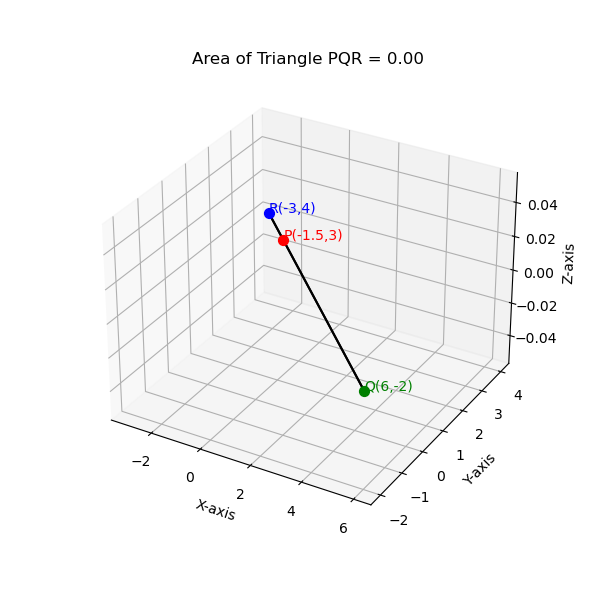
\includegraphics[height=0.5\textheight, keepaspectratio]{figs/fig4.png}
    \label{figure_1}
\end{figure}
 


\end{document}